\documentclass[tikz,border=1.35mm]{standalone}

\definecolor{fvmadaptedge}{HTML}{8A7E7E}
\usetikzlibrary{arrows.meta}

\definecolor{externalface}{HTML}{8FB9E8}
\definecolor{splitred}{HTML}{AF2525}
\definecolor{centroidgreen}{HTML}{0E8814}

% Face-based isotropic refinement scaffold for an irregular eight-faced
% polyhedral cell. Face centroids connect to edge midpoints in red, and face
% centroids connect to the volume centroid in green.
\begin{document}
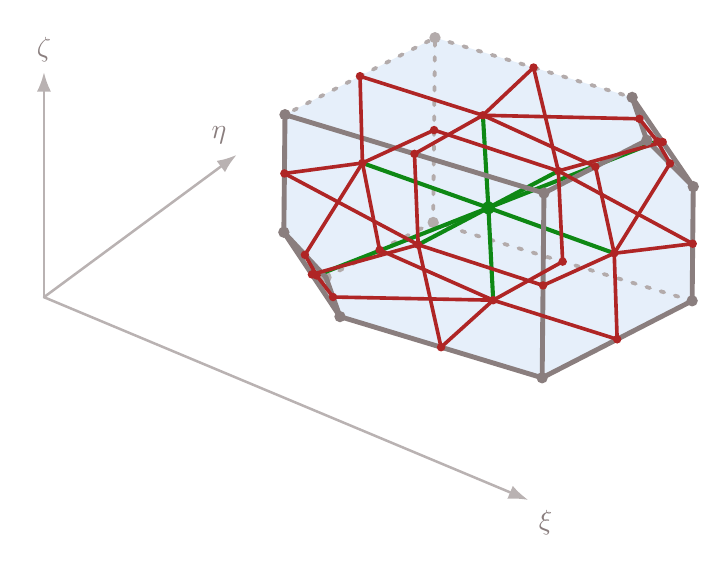
\begin{tikzpicture}[
  x={(20.3mm,-8.5mm)},
  y={(15.3mm,11.3mm)},
  z={(0mm,20mm)},
  line join=round,
  line cap=round,
  outer/.style={draw=fvmadaptedge,line width=0.62mm},
  hidden/.style={draw=fvmadaptedge!65,line width=0.48mm,loosely dotted},
  face/.style={fill=externalface,fill opacity=0.12,draw=none},
  split/.style={draw=splitred,line width=0.46mm},
  centroidedge/.style={draw=centroidgreen,line width=0.52mm},
  axis/.style={draw=fvmadaptedge!60,line width=0.32mm,-{Latex[length=2.5mm,width=1.8mm]}}
]
  % Original vertices.
  \coordinate (Oxi) at (0.3400,0.0204,0.0238);
  \coordinate (Oeta) at (0.0420,0.3000,-0.0120);
  \coordinate (Ozeta) at (-0.0200,0.0320,0.4000);
  \coordinate (B) at (1.5500,0.0930,0.1085);
  \coordinate (C) at (1.6970,1.1430,0.0665);
  \coordinate (D) at (0.1470,1.0500,-0.0420);
  \coordinate (E) at (-0.0550,0.0880,1.1000);
  \coordinate (F) at (1.4950,0.1810,1.2085);
  \coordinate (H) at (0.0920,1.1380,1.0580);
  \coordinate (Gxi) at (1.2720,1.2088,1.1406);
  \coordinate (Geta) at (1.5958,0.9010,1.1797);
  \coordinate (Gzeta) at (1.6630,1.1974,0.7465);

  % Edge midpoints.
  \coordinate (mOetaOxi) at (0.1910,0.1602,0.0059);
  \coordinate (mOetaOzeta) at (0.0110,0.1660,0.1940);
  \coordinate (mOxiOzeta) at (0.1600,0.0262,0.2119);
  \coordinate (mBOxi) at (0.9450,0.0567,0.0662);
  \coordinate (mBC) at (1.6235,0.6180,0.0875);
  \coordinate (mCD) at (0.9220,1.0965,0.0123);
  \coordinate (mDOeta) at (0.0945,0.6750,-0.0270);
  \coordinate (mBF) at (1.5225,0.1370,0.6585);
  \coordinate (mEF) at (0.7200,0.1345,1.1542);
  \coordinate (mEOzeta) at (-0.0375,0.0600,0.7500);
  \coordinate (mCGzeta) at (1.6800,1.1702,0.4065);
  \coordinate (mGetaGzeta) at (1.6294,1.0492,0.9631);
  \coordinate (mFGeta) at (1.5454,0.5410,1.1941);
  \coordinate (mGxiGzeta) at (1.4675,1.2031,0.9436);
  \coordinate (mGxiH) at (0.6820,1.1734,1.0993);
  \coordinate (mDH) at (0.1195,1.0940,0.5080);
  \coordinate (mGetaGxi) at (1.4339,1.0549,1.1602);
  \coordinate (mEH) at (0.0185,0.6130,1.0790);

  % Face centroids and volume centroid. The pentagonal-face centroids are area
  % centroids, not simple averages of their vertices.
  \coordinate (fOcut) at (0.1207,0.1175,0.1373);
  \coordinate (fBottom) at (0.8718,0.5865,0.0342);
  \coordinate (fFront) at (0.7741,0.0935,0.6235);
  \coordinate (fRight) at (1.5936,0.6334,0.6124);
  \coordinate (fBack) at (0.8644,1.1371,0.5405);
  \coordinate (fTop) at (0.7658,0.6418,1.1321);
  \coordinate (fLeft) at (0.0481,0.5941,0.5509);
  \coordinate (fGcut) at (1.5103,1.1024,1.0223);
  \coordinate (center) at (0.8203,0.6150,0.5828);

  % Offset computational-coordinate axes.
  \coordinate (Oaxis) at (-1.18,-0.42,-0.25);
  \draw[axis] (Oaxis) -- (1.85,-0.42,-0.25) node[below right,font=\normalsize,text=fvmadaptedge] {$\xi$};
  \draw[axis] (Oaxis) -- (-1.18,1.18,-0.25) node[above left,font=\normalsize,text=fvmadaptedge] {$\eta$};
  \draw[axis] (Oaxis) -- (-1.18,-0.42,1.18) node[above,font=\normalsize,text=fvmadaptedge] {$\zeta$};

  % Faint exterior faces provide depth without hiding the refinement scaffold.
  \path[face] (Oeta) -- (D) -- (H) -- (E) -- (Ozeta) -- cycle;
  \path[face] (D) -- (C) -- (Gzeta) -- (Gxi) -- (H) -- cycle;
  \path[face] (E) -- (F) -- (Geta) -- (Gxi) -- (H) -- cycle;
  \path[face] (Gxi) -- (Geta) -- (Gzeta) -- cycle;
  \path[face] (Oxi) -- (B) -- (C) -- (D) -- (Oeta) -- cycle;
  \path[face] (Oxi) -- (B) -- (F) -- (E) -- (Ozeta) -- cycle;
  \path[face] (B) -- (C) -- (Gzeta) -- (Geta) -- (F) -- cycle;
  \path[face] (Oxi) -- (Oeta) -- (Ozeta) -- cycle;

  % Hidden far-side geometry goes down before the interior construction.
  \draw[hidden] (Oeta) -- (D) -- (H) -- (E);
  \draw[hidden] (D) -- (C);
  \draw[hidden] (H) -- (Gxi);
  \fill[fvmadaptedge!65] (Oeta) circle[radius=0.72mm];
  \fill[fvmadaptedge!65] (D) circle[radius=0.72mm];
  \fill[fvmadaptedge!65] (H) circle[radius=0.72mm];

  % Face-centroid to volume-centroid connections.
  \foreach \p in {fOcut,fBottom,fFront,fRight,fBack,fTop,fLeft,fGcut} {
    \draw[centroidedge] (center) -- (\p);
  }
  \fill[centroidgreen] (center) circle[radius=0.82mm];

  % Visible exterior wireframe occludes interior centroid connections.
  \draw[outer] (Oxi) -- (B) -- (C) -- (Gzeta) -- (Geta) -- (F) -- (B);
  \draw[outer] (E) -- (F);
  \draw[outer] (E) -- (Ozeta) -- (Oxi) -- (Oeta);
  \draw[outer] (Oeta) -- (Ozeta);
  \draw[outer] (Geta) -- (Gxi) -- (Gzeta);

  % Face-centroid splits. The generic cell intentionally has triangular and
  % pentagonal faces so this figure shows mixed face valence.
  \foreach \p in {mOetaOxi,mOetaOzeta,mOxiOzeta} {
    \draw[split] (fOcut) -- (\p);
  }
  \foreach \p in {mBOxi,mBC,mCD,mDOeta,mOetaOxi} {
    \draw[split] (fBottom) -- (\p);
  }
  \foreach \p in {mBOxi,mBF,mEF,mEOzeta,mOxiOzeta} {
    \draw[split] (fFront) -- (\p);
  }
  \foreach \p in {mBC,mCGzeta,mGetaGzeta,mFGeta,mBF} {
    \draw[split] (fRight) -- (\p);
  }
  \foreach \p in {mCD,mCGzeta,mGxiGzeta,mGxiH,mDH} {
    \draw[split] (fBack) -- (\p);
  }
  \foreach \p in {mEF,mFGeta,mGetaGxi,mGxiH,mEH} {
    \draw[split] (fTop) -- (\p);
  }
  \foreach \p in {mDOeta,mDH,mEH,mEOzeta,mOetaOzeta} {
    \draw[split] (fLeft) -- (\p);
  }
  \foreach \p in {mGetaGxi,mGetaGzeta,mGxiGzeta} {
    \draw[split] (fGcut) -- (\p);
  }

  % Original vertices are #8a7e7e.
  \foreach \p in {Oxi,Ozeta,B,C,E,F,Gxi,Geta,Gzeta} {
    \fill[fvmadaptedge] (\p) circle[radius=0.72mm];
  }

  % Edge and face refinement nodes are red.
  \foreach \p in {mOetaOxi,mOetaOzeta,mOxiOzeta,mBOxi,mBC,mCD,mDOeta,
                  mBF,mEF,mEOzeta,mCGzeta,mGetaGzeta,mFGeta,
                  mGxiGzeta,mGxiH,mDH,mGetaGxi,mEH,
                  fOcut,fBottom,fFront,fRight,fBack,fTop,fLeft,fGcut} {
    \fill[splitred] (\p) circle[radius=0.54mm];
  }
\end{tikzpicture}
\end{document}
